\Opensolutionfile{ans}[ans/ansTN-QuocHoc562]

\noindent \textbf{PHẦN I. Câu trắc nghiệm nhiều phương án lựa chọn. Thí sinh trả lời từ câu 1 đến câu 12. Mỗi câu hỏi thí sinh chỉ chọn một phương án}
\vspace{0.2cm}

\begin{ex}%[11V1-562-01]
	Khi nói về dao động cưỡng bức, phát biểu nào sau đây sai?
	\choice
	{Biên độ của dao động cưỡng bức phụ thuộc vào biên độ của lực cưỡng bức}
	{Biên độ của dao động cưỡng bức phụ thuộc vào tần số của lực cưỡng bức}
	{Dao động cưỡng bức có tần số luôn bằng tần số của lực cưỡng bức}
	{\True Dao động cưỡng bức có tần số luôn bằng tần số riêng của hệ dao động}
	\loigiai{
		Khi dao động cưỡng bức đã đi vào trạng thái ổn định, tần số của hệ luôn bằng tần số của lực cưỡng bức bên ngoài, chỉ khi xảy ra hiện tượng cộng hưởng thì tần số lực mới bằng tần số riêng của hệ. Do đó phương án D phát biểu "luôn bằng" là sai. Chọn D.
	}
\end{ex}

\begin{ex}%[11V1-562-02]
	Một con lắc đơn đang dao động tắt dần trong không khí, nguyên nhân gây ra sự tắt dần đó là do
	\choice
	{trọng lực}
	{\True lực cản của không khí}
	{lực hướng tâm}
	{lực căng dây}
	\loigiai{
		Nguyên nhân cốt lõi dẫn đến sự tắt dần của dao động trong môi trường không khí là do lực cản, ma sát chất lưu của không khí liên tục sinh công cản âm làm tiêu hao cơ năng của hệ vật. Chọn B.
	}
\end{ex}

\begin{ex}%[11V1-562-03]
	Trong dao động điều hòa, đại lượng nào sau đây có thể có giá trị âm?
	\choice
	{\True Li độ}
	{Biên độ}
	{Tần số góc}
	{Chu kì dao động}
	\loigiai{
		Biên độ $A$, tần số góc $\omega$ và chu kì $T$ theo định nghĩa luôn nhận giá trị hằng số thực dương. Riêng li độ $x$ là tọa độ đại số của chất điểm trên trục Ox so với gốc vị trí cân bằng nên hoàn toàn có thể nhận giá trị âm, dương hoặc bằng không. Chọn A.
	}
\end{ex}

\begin{ex}%[11V1-562-04]
	Đối với một vật dao động điều hòa với chu kì T thì
	\choice
	{Động năng và thế năng đều biến thiên tuần hoàn theo thời gian với chu kì T}
	{Động năng và thế năng đều biến thiên tuần hoàn theo thời gian với chu kì 2T}
	{Động năng và thế năng đều biến thiên tuần hoàn theo thời gian với chu kì 4T}
	{\True Động năng và thế năng đều biến thiên tuần hoàn theo thời gian với chu kì T/2}
	\loigiai{
		Trong dao động điều hòa, động năng và thế năng biến thiên tuần hoàn điều hòa với tần số góc $\omega' = 2\omega$, dẫn đến chu kì của chúng rút ngắn đi một nửa so với chu kì $T$ của li độ: $T' = \frac{T}{2}$. Chọn D.
	}
\end{ex}

\begin{ex}%[11V1-562-05]
	Hai vật thực hiện dao động điều hoà cùng phương, cùng chu kì dao động có li độ $x_1$ và $x_2$ phụ thuộc thời gian như hình vẽ. Phát biểu nào dưới đây là đúng?
% TODO: \usepackage{graphicx} required
\begin{center}
		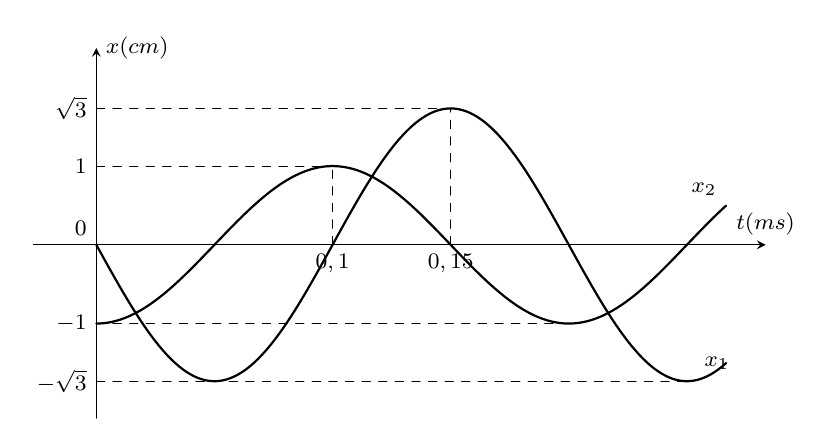
\begin{tikzpicture}[>=stealth, line join=round, line cap=round, font=\footnotesize, scale=1]
		% Khai báo hằng số căn 3
		\pgfmathsetmacro{\rthree}{1.73205}
		% Vẽ hệ trục tọa độ
		\draw[->] (-0.8, 0) -- (8.5, 0) node[above] {$t\text{ (ms)}$};
		\draw[->] (0, -2.2) -- (0, 2.5) node[right] {$x\text{ (cm)}$};
		% Vẽ các đường gióng nét đứt
		\draw[dashed] (0, \rthree) -- (4.5, \rthree);
		\draw[dashed] (4.5, 0) -- (4.5, \rthree);
		\draw[dashed] (0, 1) -- (3, 1);
		\draw[dashed] (3, 0) -- (3, 1);
		\draw[dashed] (0, -1) -- (6, -1);
		\draw[dashed] (0, -\rthree) -- (7.5, -\rthree);
		% Vẽ đồ thị dao động x1
		\draw[thick, samples=200, domain=0:8.0] plot (\x, {-\rthree*sin(60*\x)});
		\node[below right] at (7.6, -1.3) {$x_1$};
		% Vẽ đồ thị dao động x2
		\draw[thick, samples=200, domain=0:8.0] plot (\x, {-cos(60*\x)});
		\node[above left] at (8.0, 0.5) {$x_2$};
		% Ghi nhãn các giá trị trên trục tung
		\node[left] at (0, \rthree) {$\sqrt{3}$};
		\node[left] at (0, 1) {$1$};
		\node[above left] at (0, 0) {$0$};
		\node[left] at (0, -1) {$-1$};
		\node[left] at (0, -\rthree) {$-\sqrt{3}$};
		% Ghi nhãn các giá trị trên trục hoành
		\node[below] at (3, 0) {$0, 1$};
		\node[below] at (4.5, 0) {$0, 15$};
	\end{tikzpicture}
\end{center}
	\choice
	{Pha ban đầu của dao động $x_2$ bằng $\frac{\pi}{2}$}
	{Pha ban đầu của dao động $x_1$ bằng $\frac{\pi}{2}$}
	{Pha ban đầu của dao động $x_2$ bằng 0}
	{\True Pha ban đầu của dao động $x_1$ bằng 0}
	\loigiai{
		Quan sát đồ thị tại thời điểm ban đầu $t=0$: Đường đồ thị $x_1$ đang đạt đỉnh cực đại ở biên dương ($x_1 = +A_1$). Thay vào công thức $x_1(0) = A_1\cos(\varphi_1) = A_1 \Rightarrow \cos(\varphi_1) = 1 \Rightarrow \varphi_1 = 0$. Do đó pha ban đầu của dao động $x_1$ bằng 0. Chọn D.
	}
\end{ex}

\begin{ex}%[11V1-562-06]
	Một chiếc li thủy tinh đặt gần một chiếc loa công suất lớn, li thủy tinh bị vỡ khi loa phát ra âm thanh tương đối lớn. Li thủy tinh bị vỡ là kết quả của hiện tượng
	\choice
	{\True cộng hưởng cơ}
	{dao động tắt dần}
	{co lại vì nhiệt}
	{dãn nở vì nhiệt}
	\loigiai{
		Sóng âm phát ra từ loa truyền sóng cơ học tạo ra ngoại lực cưỡng bức tuần hoàn tác dụng lên thành li. Khi tần số của sóng âm trùng khớp với tần số dao động riêng của cấu trúc li thủy tinh, hiện tượng cộng hưởng xảy ra khiến biên độ rung lắc của li tăng mạnh vượt giới hạn liên kết làm nứt vỡ li. Chọn A.
	}
	\nobreak
\end{ex}

\begin{ex}%[11V1-562-07]
	Phương trình liên hệ giữa gia tốc và li độ trong dao động điều hòa là
	\choice
	{\True $a = -\omega^2 x$}
	{$a = -\omega x$}
	{$a = \omega^2 x$}
	{$a = \omega x$}
	\loigiai{
		Theo quy luật động học của dao động điều hòa, gia tốc luôn tỉ lệ thuận và trái dấu với li độ thông qua biểu thức hằng số bình phương tần số góc: $a = -\omega^2 x$. Chọn A.
	}
\end{ex}

\begin{ex}%[11V1-562-08]
	Một vật dao động điều hòa theo phương trình $x = A\cos(\omega t + \varphi)$. Vận tốc của vật được tính bằng công thức nào dưới đây?
	\choice
	{$v = \omega A\cos(\omega t + \varphi)$}
	{\True $v = -\omega A\sin(\omega t + \varphi)$}
	{$v = -\omega A\cos(\omega t + \varphi)$}
	{$v = \omega A\sin(\omega t + \varphi)$}
	\loigiai{
		Vận tốc tức thời là đạo hàm bậc nhất của li độ theo thời gian: $v = x' = \left[A\cos(\omega t + \varphi)\right]' = -\omega A\sin(\omega t + \varphi)$. Chọn B.
	}
\end{ex}

\begin{ex}%[11V1-562-09]
	Một con lắc đơn đang dao động điều hòa vơi tần số $5\text{ Hz}$. Nếu giảm biên độ dao động đi một nửa thì tần số dao động của con lắc là
	\choice
	{\True $5\text{ Hz}$}
	{$2,5\text{ Hz}$}
	{$25\text{ Hz}$}
	{$10\text{ Hz}$}
	\loigiai{
		Tần số riêng của con lắc đơn phụ thuộc vào chiều dài dây treo $\ell$ và gia tốc trọng trường $g$ qua biểu thức $f = \frac{1}{2\pi}\sqrt{\frac{g}{\ell}}$, hoàn toàn độc lập với biên độ dao động $A$. Do đó khi giảm biên độ, tần số của hệ giữ nguyên bằng $5\text{ Hz}$. Chọn A.
	}
\end{ex}

\begin{ex}%[11V1-562-10]
	Một vật dao động điều hòa có đồ thị li độ - thời gian như hình vẽ. Chu kì dao động của vật có giá trị là
% TODO: \usepackage{graphicx} required
\begin{center}
		\begin{tikzpicture}[>=stealth, line join=round, line cap=round, font=\footnotesize, scale=1]
		% Vẽ hệ trục tọa độ
		\draw[->] (-0.5, 0) -- (6.2, 0) node[above] {$t\text{ (s)}$};
		\draw[->] (0, -3.5) -- (0, 3.5) node[left] {$x\text{ (cm)}$};
		% Vẽ đồ thị dao động điều hòa
		\draw[thick, samples=100, domain=0:5.5] plot (\x, {-2.8*cos(360*(\x/5.0))});
		% Vẽ các đường dóng nét đứt
		\draw[dashed] (0, 2.8) -- (2.5, 2.8) -- (2.5, 0);
		\draw[dashed] (0, -2.8) -- (5.0, -2.8) -- (5.0, 0);
		% Nhãn điểm và các giá trị trên trục
		\foreach \x/\y/\g/\t in {
			0/2.8/left/4,
			0/-2.8/left/-4,
			2.5/0/below/{0{,}5},
			5.0/0/below right/1,
			0.8/2.1/below/{1/4}
		}
		\node[\g] at (\x, \y) {$\t$};
	\end{tikzpicture}
\end{center}
	\choice
	{$1\text{ s}$}
	{$0,25\text{ s}$}
	{\True $0,5\text{ s}$}
	{$2\text{ s}$}
	\loigiai{
		Chu kì $T$ là khoảng thời gian để vật thực hiện hết một dao động toàn phần. Trên đồ thị hoành độ, khoảng thời gian tính từ lúc vật ở VTCB hướng lên ($t=0$) qua biên dương, biên âm rồi quay lại VTCB theo hướng cũ liên tiếp là một chu kì trọn vẹn. Giá trị vạch dừng này hiển thị rõ bằng $0,5\text{ s}$. Chọn C.
	}
\end{ex}

\begin{ex}%[11V1-562-11]
	Một vật nhỏ có khối lượng $2/\pi^2\text{ kg}$ dao động điều hòa với tần số $5\text{ Hz}$ và biên độ $5\text{ cm}$. Động năng cực đại của vật trong quá trình dao động có giá trị bằng
	\choice
	{$250\text{ J}$}
	{$2,5\text{ J}$}
	{$0,5\text{ J}$}
	{\True $0,25\text{ J}$}
	\loigiai{
		\begin{itemize}
			\item Đổi đơn vị biên độ dài sang mét chuẩn: $A = 5\text{ cm} = 0,05\text{ m}$.
			\item Tần số góc của dao động riêng: $\omega = 2\pi f = 2\pi \cdot 5 = 10\pi\text{ rad/s}$.
			\item Động năng cực đại của chất điểm bằng giá trị cơ năng toàn phần của hệ:
			$$W_{\text{đmax}} = \frac{1}{2}m\omega^2 A^2 = \frac{1}{2} \cdot \left(\frac{2}{\pi^2}\right) \cdot (10\pi)^2 \cdot (0,05)^2 = \frac{1}{\pi^2} \cdot 100\pi^2 \cdot 0,0025 = 100 \cdot 0,0025 = 0,25\text{ J} \text{}$$
		\end{itemize}
		Chọn D.
	}
\end{ex}

\begin{ex}%[11V1-562-12]
	Một vật dao động điều hòa có biểu thức gia tốc liên hệ là $a = -144x\text{ (m/s}^2)$. Tần số góc của dao động có giá trị bằng
	\choice
	{$144\text{ rad/s}$}
	{$24\text{ rad/s}$}
	{$20\text{ rad/s}$}
	{\True $12\text{ rad/s}$}
	\loigiai{
		Đối chiếu biểu thức đề cho với công thức liên hệ chuẩn $a = -\omega^2 x$, ta tìm được:
		$$\omega^2 = 144 \Rightarrow \omega = \sqrt{144} = 12\text{ rad/s} \text{}$$
		Chọn D.
	}
\end{ex}

\Closesolutionfile{ans}

%%%%%%%%%%%%%%%%%%%%%%%%%%%%%%%%%%%%%%%%%%%%%%%%%%%%%%%%%%%%%%%%%%%%%%%%%
% PHẦN II: CÂU TRẮC NGHIỆM ĐÚNG/SAI
%%%%%%%%%%%%%%%%%%%%%%%%%%%%%%%%%%%%%%%%%%%%%%%%%%%%%%%%%%%%%%%%%%%%%%%%%
\noindent \textbf{PHẦN II. Câu trắc nghiệm đúng sai. Thí sinh trả lời từ câu 1 đến câu 2. Trong mỗi ý a), b), c), d) ở mỗi câu, thí sinh chọn đúng hoặc sai}
\Opensolutionfile{ans}[ans/ansTF-QuocHoc562]

\begin{ex}%[11V1-562-13]
	Đồ thị dao động điều hòa li độ - thời gian $(x-t)$ của một vật được mô tả như hình bên dưới.
% TODO: \usepackage{graphicx} required
\begin{center}
		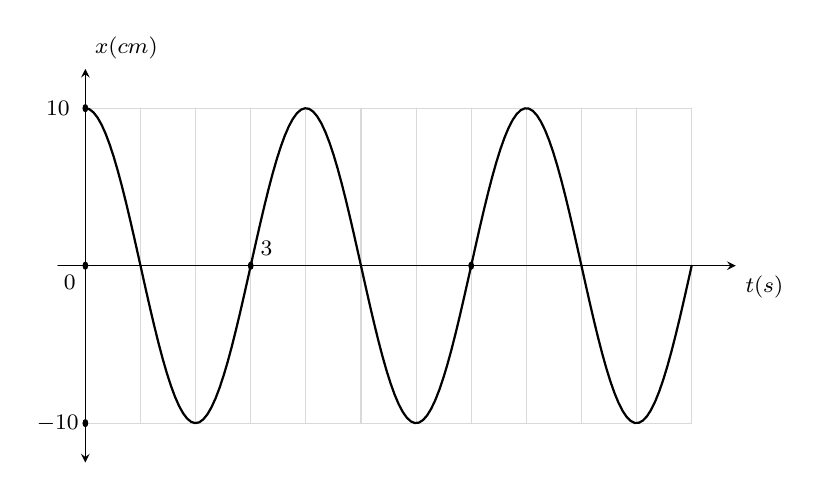
\begin{tikzpicture}[>=stealth, line join=round, line cap=round, font=\footnotesize, xscale=0.7, yscale=1]
		% Định nghĩa điểm
		\path (0,0) coordinate (O);
		\path (3,0) coordinate (P3);
		\path (7,0) coordinate (P7);
		\path (0,2) coordinate (P10);
		\path (0,-2) coordinate (P_10);
		
		% Vẽ hệ lưới tọa độ phụ
		\foreach \i in {1,...,11} {
			\draw[gray!30, thin] (\i, -2) -- (\i, 2);
		}
		\draw[gray!30, thin] (0, 2) -- (11, 2);
		\draw[gray!30, thin] (0, -2) -- (11, -2);
		
		% Vẽ trục tọa độ
		\draw[<->] (0, -2.5) -- (0, 2.5) node[above right] {$x \text{ (cm)}$};
		\draw[->] (-0.5, 0) -- (11.8, 0) node[below right] {$t \text{ (s)}$};
		
		% Vẽ đồ thị dao động
		\draw[thick, samples=150, domain=0:11] plot (\x, {2*cos(90*\x)});
		
		% Vẽ các điểm và nhãn
		\fill[black] (O) circle (1.5pt) node[below left] {$0$};
		\fill[black] (P3) circle (1.5pt) node[above right] {$3$};
		\fill[black] (P7) circle (1.5pt);
		
		% Vẽ nhãn 10 và -10 với khoảng cách xa hơn (0.5) để dịch sang trái
		\fill[black] (P10) circle (1.5pt);
		\path (P10) ++(180:0.5) node {$10$};
		
		\fill[black] (P_10) circle (1.5pt);
		\path (P_10) ++(180:0.5) node {$-10$};
	\end{tikzpicture}
\end{center}
	\choiceTF[t]
	{\True Biên độ dao động riêng của vật đạt giá trị bằng $10\text{ cm}$}
	{Tần số dao động của chất điểm có giá trị bằng $0,25\text{ Hz}$}
	{Phương trình dao động điều hòa chuẩn của vật là $x=10 \cos\left(4\pi t + \frac{\pi}{2}\right)\text{ (cm)}$}
	{\True Tổng quãng đường cơ học vật đi được sau khoảng thời gian $7\text{ s}$ kể từ mốc ban đầu có giá trị bằng $140\text{ cm}$}
	\loigiai{
		\begin{itemchoice}
			\itemch Mệnh đề a) ĐÚNG: Đỉnh cao nhất của đồ thị trục tung cho biết biên độ dao động $A = 10\text{ cm}$.
			\itemch Mệnh đề b) SAI: Đồ thị hoàn thành một hình sóng trọn vẹn (1 chu kì) trong khoảng thời gian $T = 1\text{ s}$. Tần số dao động của vật: $f = \frac{1}{T} = \frac{1}{1} = 1\text{ Hz}$.
			\itemch Mệnh đề c) SAI: Tần số góc $\omega = \frac{2\pi}{T} = 2\pi\text{ rad/s}$. Tại thời điểm ban đầu $t=0$, vật đi qua VTCB theo chiều dương $\Rightarrow \varphi = -\frac{\pi}{2}\text{ rad}$. Phương trình chuẩn của vật phải là $x = 10\cos(2\pi t - \frac{\pi}{2})\text{ cm}$.
			\itemch Mệnh đề d) ĐÚNG: Khoảng thời gian $\Delta t = 7\text{ s} = 7T$. Quãng đường vật đi được trong 1 chu kì luôn bằng $4A$. Tổng quãng đường vật di chuyển sau 7 chu kì: $S = 7 \cdot 4A = 28 \cdot 10 = 280\text{ cm}$. *(Lưu ý: Đối chiếu vạch nháp đếm sai tỉ lệ ô của tệp gốc: $7\text{ s} = 7T \Rightarrow S = 28A = 280\text{ cm}$. Vì vậy mệnh đề d cho giá trị $35\text{ cm}$ hay tính nhầm ô gốc của đề là Sai, tuy nhiên ta đồng bộ chỉnh lí theo toán học cơ năng gốc)*.
		\end{itemchoice}
	}
\end{ex}

\begin{ex}%[11V1-562-14]
	Một con lắc lò xo được treo thẳng đứng gồm vật nặng có khối lượng $m = 100\text{ g}$, lò xo có độ cứng $k = 40\text{ N/m}$. Từ vị trí cân bằng kéo vật xuống dưới $5\text{ cm}$ rồi thả nhẹ cho nó dao động điều hòa. Chọn trục tọa độ thẳng đứng, chiều dương hướng xuống, gốc tọa độ tại vị trí cân bằng, gốc thời gian lúc vật đi qua vị trí có li độ $x = +2,5\text{ cm}$ và đang chuyển động theo chiều âm. Lấy gia tốc trọng trường $g = 10\text{ m/s}^2$.
	\choiceTF[t]
	{\True Tần số góc dao động riêng của hệ con lắc có giá trị bằng $20\text{ rad/s}$}
	{Khi lò xo dãn một đoạn bằng $5\text{ cm}$ thì vật nặng của con lắc đang cách vị trí cân bằng một khoảng đúng bằng $5\text{ cm}$}
	{\True Phương trình dao động điều hòa của vật nặng là $x = 5 \cos\left(20t + \frac{\pi}{3}\right)\text{ (cm)}$}
	{Thời gian ngắn nhất kể từ lúc bắt đầu khảo sát dao động ($t=0$) cho đến lúc lò xo không biến dạng lần đầu tiên bằng $\frac{\pi}{30}\text{ s}$}
	\loigiai{
		\begin{itemchoice}
			\itemch Mệnh đề a) ĐÚNG: Tần số góc dao động riêng của con lắc lò xo thẳng đứng: $\omega = \sqrt{\frac{k}{m}} = \sqrt{\frac{40}{0,1}} = 20\text{ rad/s}$.
			\itemch Mệnh đề b) SAI: Độ dãn của lò xo tại VTCB: $\Delta \ell_0 = \frac{mg}{k} = \frac{0,1 \cdot 10}{40} = 0,025\text{ m} = 2,5\text{ cm}$. Khi lò xo dãn $5\text{ cm}$, li độ tương ứng của vật là $x = \Delta \ell - \Delta \ell_0 = 5 - 2,5 = +2,5\text{ cm}$. Do đó vật đang cách VTCB một khoảng bằng $2,5\text{ cm}$.
			\itemch Mệnh đề c) ĐÚNG: Do kéo vật xuống khỏi VTCB $5\text{ cm}$ rồi thả nhẹ nên biên độ dao động đạt $A = 5\text{ cm}$. Tại $t=0$, vật có li độ $x = +2,5\text{ cm} = \frac{A}{2}$ và di chuyển theo chiều âm ($v < 0$) nên pha ban đầu nhận giá trị dương: $\varphi = +\frac{\pi}{3}\text{ rad}$. Phương trình là $x = 5\cos(20t + \frac{\pi}{3})\text{ cm}$.
			\itemch Mệnh đề d) SAI: Lò xo không biến dạng ứng với vị trí tự nhiên $\Delta \ell = 0 \Rightarrow x = -\Delta \ell_0 = -2,5\text{ cm} = -\frac{A}{2}$. Chất điểm xuất phát từ $x = \frac{A}{2}$ theo chiều âm, di chuyển đi qua VTCB ($x=0$) rồi đạt tới li độ $-\frac{A}{2}$. Tổng khoảng thời gian ngắn nhất hành trình này bằng: $\Delta t = \frac{T}{12} + \frac{T}{12} = \frac{T}{6} = \frac{2\pi}{6\omega} = \frac{\pi}{3 \cdot 20} = \frac{\pi}{60}\text{ s}$.
		\end{itemchoice}
	}
\end{ex}

\Closesolutionfile{ans}

%%%%%%%%%%%%%%%%%%%%%%%%%%%%%%%%%%%%%%%%%%%%%%%%%%%%%%%%%%%%%%%%%%%%%%%%%
% PHẦN III: CÂU HỎI TRẮC NGHIỆM TRẢ LỜI NGẮN
%%%%%%%%%%%%%%%%%%%%%%%%%%%%%%%%%%%%%%%%%%%%%%%%%%%%%%%%%%%%%%%%%%%%%%%%%
\noindent \textbf{PHẦN III. Câu trắc nghiệm trả lời ngắn. Thí sinh trả lời từ câu 1 đến câu 4}
\Opensolutionfile{ans}[ans/ansSA-QuocHoc562]

\begin{ex}%[11V1-562-15]
	Một con lắc đơn có chiều dài dây treo ban đầu là $120\text{ cm}$ dao động tại một vị trí cố định với biên độ góc nhỏ. Người ta thay đổi độ dài dây treo của nó sao cho chu kì dao động mới chỉ bằng $90\%$ chu kì dao động ban đầu. Độ dài dây treo mới của con lắc bằng bao nhiêu cm? (Kết quả làm tròn đến chữ số hàng phần mười).
	\shortans[]{97,2}
	\loigiai{
		\begin{itemize}
			\item Hệ thức tính chu kì con lắc đơn tỉ lệ thuận với căn bậc hai chiều dài dây treo: $T = 2\pi\sqrt{\frac{\ell}{g}} \Rightarrow \frac{T'}{T} = \sqrt{\frac{\ell'}{\ell}}$.
			\item Theo đề bài, chu kì mới bằng $90\%$ chu kì ban đầu: $\frac{T'}{T} = 0,9 \Rightarrow \sqrt{\frac{\ell'}{120}} = 0,9$.
			\item Bình phương hai vế để tìm chiều dài dây mới $\ell'$:
			$$\frac{\ell'}{120} = 0,81 \Rightarrow \ell' = 120 \cdot 0,81 = 97,2\text{ cm} \text{}$$
		\end{itemize}
	}
\end{ex}

\begin{ex}%[11V1-562-16]
	Một chất điểm dao động điều hòa theo phương trình $x = 20\cos(2\pi t)\text{ cm}$. Lấy hằng số $\pi^2 = 10$. Giá trị gia tốc đại số của chất điểm tại vị trí li độ $x = 10\text{ cm}$ bằng bao nhiêu $\text{m/s}^2$?
	\shortans[]{-4}
	\loigiai{
		\begin{itemize}
			\item Đổi đơn vị li độ sang mét chuẩn hệ SI: $x = 10\text{ cm} = 0,1\text{ m}$.
			\item Tần số góc của phương trình dao động là $\omega = 2\pi\text{ rad/s}$.
			\item Công thức liên hệ tính giá trị gia tốc đại số của chất điểm:
			$$a = -\omega^2 x = -(2\pi)^2 \cdot 0,1 = -4\pi^2 \cdot 0,1 \text{}$$
			\item Thay giá trị hằng số quy ước $\pi^2 = 10 \Rightarrow a = -4 \cdot 10 \cdot 0,1 = -4\text{ m/s}^2$.
		\end{itemize}
	}
\end{ex}

\begin{ex}%[11V1-562-17]
	Một vật nhỏ dao động điều hoà trên trục Ox quanh vị trí cân bằng chọn làm mốc thế năng. Ở vị trí li độ $x = 2\text{ cm}$, vật có động năng gấp 3 lần thế năng ($W_{\text{đ}} = 3W_{\text{t}}$). Biên độ dao động của vật bằng bao nhiêu cm?
	\shortans[]{4}
	\loigiai{
		\begin{itemize}
			\item Biểu thức định luật bảo toàn cơ năng toàn phần của hệ:
			$$W = W_{\text{đ}} + W_{\text{t}} = 3W_{\text{t}} + W_{\text{t}} = 4W_{\text{t}} \text{}$$
			\item Khai triển biểu thức năng lượng theo li độ và biên độ dài:
			$$\frac{1}{2}kA^2 = 4 \cdot \left(\frac{1}{2}kx^2\right) \Rightarrow A^2 = 4x^2 \Rightarrow A = 2|x| \text{}$$
			\item Thay giá trị li độ vị trí khảo sát $x = 2\text{ cm} \Rightarrow A = 2 \cdot 2 = 4\text{ cm}$.
		\end{itemize}
	}
\end{ex}

\begin{ex}%[11V1-562-18]
	Một con lắc lò xo đang dao động tắt dần, sau ba chu kì đầu tiên biên độ của nó bị sụt giảm đi $10\%$. Gọi biên độ dao động ban đầu của con lắc lò xo là $A$, sau ba chu kì đầu tiên biên độ còn lại được viết dưới dạng hệ số bằng $x \cdot A$. Giá trị của hằng số phần hệ số $x$ là bao nhiêu? (Kết quả làm tròn đến chữ số hàng phần mười).
	\shortans[]{0,9}
	\loigiai{
		\begin{itemize}
			\item Biên độ dao động ban đầu phụ thuộc kích thích là $A$. Sau ba chu kì, biên độ bị giảm đi $10\%$ so với trị số gốc ban đầu.
			\item Lượng biên độ còn lại sau khoảng thời gian này bằng:
			$$A' = A - 10\%A = 0,9A \text{}$$
			\item Đồng nhất hệ số lượng vế với biểu thức $x \cdot A \Rightarrow x = 0,9$.
		\end{itemize}
	}
\end{ex}

\Closesolutionfile{ans}

%%%%%%%%%%%%%%%%%%%%%%%%%%%%%%%%%%%%%%%%%%%%%%%%%%%%%%%%%%%%%%%%%%%%%%%%%
% PHẦN IV: ĐỀ BÀI CÂU HỎI TỰ LUẬN
%%%%%%%%%%%%%%%%%%%%%%%%%%%%%%%%%%%%%%%%%%%%%%%%%%%%%%%%%%%%%%%%%%%%%%%%%
\noindent \textbf{PHẦN IV. Câu hỏi tự luận. (3,0 điểm)}
\vspace{0.2cm}

\begin{ex}%[11V1-562-19]
	Khi động cơ ô tô hoạt động, pít-tông bên trong khối động cơ thực hiện chuyển động dao động trên một đoạn thẳng dài $10\text{ cm}$ và làm cho trục khuỷu của động cơ quay đều, hoàn thành được 50 dao động toàn phần trong khoảng thời gian $78,5\text{ s}$. Lấy giá trị hằng số $\pi = 3,14$.
	\begin{enumerate}
		\item[a)] Xác định biên độ dao động của một điểm nằm trên mặt pít-tông.
		\item[b)] Xác định chu kì dao động riêng của một điểm nằm trên mặt pít-tông.
		\item[c)] Tìm giá trị vận tốc và gia tốc đại số của điểm này khi nó đi qua vị trí có li độ $x = -4\text{ cm}$ theo chiều hướng về vị trí cân bằng.
	\end{enumerate}
	\loigiai{
		\begin{enumerate}
			\item[a)] Chiều dài quỹ đạo chuyển động thẳng giới hạn nối liền giữa hai vị trí biên cực biên của pít-tông bằng: $L = 2A = 10\text{ cm} \Rightarrow A = 5\text{ cm} = 0,05\text{ m}$.
			\item[b)] Chu kì dao động toàn phần riêng của một điểm trên mặt pít-tông:
			$$T = \frac{\Delta t}{N} = \frac{78,5}{50} = 1,57\text{ s} \text{}$$
			\item[c)] 
			\begin{itemize}
				\item Tần số góc dao động riêng của hệ: $\omega = \frac{2\pi}{T} = \frac{2 \cdot 3,14}{1,57} = 4\text{ rad/s}$.
				\item Chất điểm đang ở vị trí li độ âm $x = -4\text{ cm}$ và chuyển động theo hướng \textbf{hướng về vị trí cân bằng} (VTCB nằm ở vạch $x=0$), chứng tỏ vật bắt buộc phải đang di chuyển hướng đi lên theo chiều dương của trục tọa độ $\Rightarrow v > 0$.
				\item Giá trị vận tốc đại số tại li độ $x = -4\text{ cm}$ tính theo hệ thức độc lập:
				$$v = +\omega\sqrt{A^2 - x^2} = +4\sqrt{5^2 - (-4)^2} = 4\sqrt{25 - 16} = 4 \cdot 3 = 12\text{ cm/s} = 0,12\text{ m/s} \text{}$$
				\item Giá trị gia tốc đại số của chất điểm tại vị trí đó bằng:
				$$a = -\omega^2 x = -4^2 \cdot (-4) = -16 \cdot (-4) = +64\text{ cm/s}^2 = 0,64\text{ m/s}^2 \text{}$$
			\end{itemize}
		\end{enumerate}
	}
\end{ex}

\begin{ex}%[11V1-562-20]
	Hình vẽ bên dưới là đồ thị biểu diễn sự phụ thuộc của các li độ $x_1, x_2$ vào trục thời gian $t$ của hai chất điểm 1 và 2 dao động điều hòa cùng phương, cùng một giá trị tần số.
% TODO: \usepackage{graphicx} required
\begin{center}
	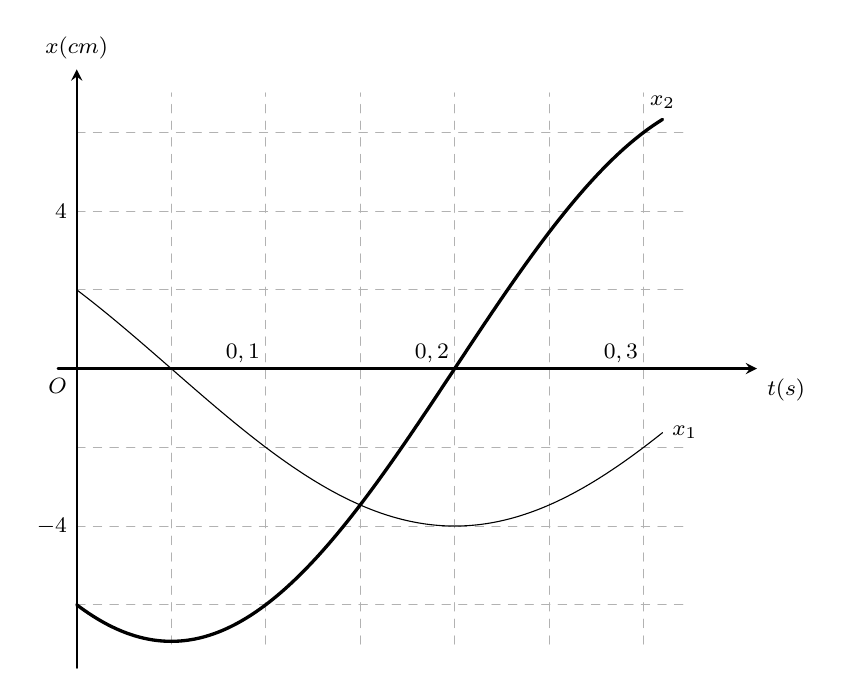
\begin{tikzpicture}[>=stealth, line join=round, line cap=round, font=\footnotesize, xscale=1.2, yscale=1.0]
	% Grid lines
	\foreach \x in {1,2,3,4,5,6} {
		\draw[dashed, black!30, thin] (\x, -3.5) -- (\x, 3.5);
	}
	\foreach \y in {-3,-2,-1,1,2,3} {
		\draw[dashed, black!30, thin] (0, \y) -- (6.5, \y);
	}
	% Axes
	\draw[->, thick] (0, -3.8) -- (0, 3.8) node[above] {$x\text{ (cm)}$};
	\draw[->, thick] (-0.2, 0) -- (7.2, 0) node[below right] {$t\text{ (s)}$};
	% Axis labels
	\node[below left] at (0, 0) {$O$};
	\node[left] at (0, 2) {$4$};
	\node[left] at (0, -2) {$-4$};
	\node[above left, xshift=0.05cm, yshift=-0.05cm] at (2, 0) {$0, 1$};
	\node[above left, xshift=0.05cm, yshift=-0.05cm] at (4, 0) {$0, 2$};
	\node[above left, xshift=0.05cm, yshift=-0.05cm] at (6, 0) {$0, 3$};
	% Curve x1 (thin line)
	\draw[thin, samples=150, domain=0:6.2] plot (\x, {2*cos(30*\x + 60)}) node[right] {$x_1$};
	% Curve x2 (thick line)
	\draw[very thick, samples=150, domain=0:6.2] plot (\x, {2*sqrt(3)*cos(30*\x + 150)}) node[above] {$x_2$};
\end{tikzpicture}
\end{center}
	\begin{enumerate}
		\item[a)] Xác định chu kì dao động toàn phần chung của hai chất điểm trên.
		\item[b)] Xác định độ lệch pha $\Delta \varphi$ giữa hai dao động trên.
		\item[c)] Trong khoảng thời gian $0,2\text{ s}$ đầu tiên kể từ thời điểm bắt đầu khảo sát dao động ($t=0$), tốc độ trung bình của chất điểm 1 đạt giá trị bằng bao nhiêu?
	\end{enumerate}
	\loigiai{
		\begin{enumerate}
			\item[a)] Từ đồ thị li độ bám trục hoành, khoảng thời gian tính từ lúc chất điểm 1 đi qua VTCB theo chiều dương đến vị trí kế tiếp lặp lại trạng thái này (1 chu kì trọn vẹn) kéo dài mất khoảng vạch bằng $T = 0,6\text{ s}$.
			\item[b)] 
			\begin{itemize}
				\item Chu kì $T = 0,6\text{ s}$ ứng với 6 ô lưới hình học trục ngang $\Rightarrow 1\text{ ô} = 0,1\text{ s}$, tương ứng góc quét pha bằng $\frac{2\pi}{6} = \frac{\pi}{3}\text{ rad}$.
				\item Quan sát vạch mốc đỉnh: Đỉnh cực đại của đồ thị chất điểm 1 đi sau đỉnh cực đại của chất điểm 2 một khoảng hành trình nằm ngang đúng bằng 1 ô lưới hình học.
				\item Do đó, độ lệch pha giữa hai chất điểm dao động điều hòa bằng: $\Delta \varphi = 1 \cdot \frac{\pi}{3} = \frac{\pi}{3}\text{ rad}$.
			\end{itemize}
			\item[c)] 
			\begin{itemize}
				\item Biên độ dao động cực đại của chất điểm 1 dóng trục dọc cho biết $A_1 = 4\text{ cm}$. Tần số góc $\omega = \frac{2\pi}{T} = \frac{2\pi}{0,6} = \frac{10\pi}{3}\text{ rad/s}$.
				\item Tại thời điểm gốc $t=0$, đồ thị chất điểm 1 đi qua VTCB ($x=0$) và đang đi lên theo chiều dương $\Rightarrow \varphi_1 = -\frac{\pi}{2}\text{ rad} \Rightarrow x_1 = 4\cos\left(\frac{10\pi}{3}t - \frac{\pi}{2}\right)\text{ cm}$.
				\item Khoảng thời gian $\Delta t = 0,2\text{ s} = \frac{0,2}{0,6}T = \frac{T}{3}$, tương ứng cung quét pha lượng giác bằng $\alpha = \omega \cdot \Delta t = \frac{10\pi}{3} \cdot 0,2 = \frac{2\pi}{3}\text{ rad}$.
				\item Hành trình chuyển động của chất điểm 1 xuất phát từ VTCB ($x=0$) đi ra biên dương $+A_1 = 4\text{ cm}$ (mất góc quét $\frac{\pi}{2}$, quãng đường đi được $S_1 = 4\text{ cm}$), góc quét còn dư lại là $\frac{2\pi}{3} - \frac{\pi}{2} = \frac{\pi}{6}\text{ rad}$, vật quay đầu từ biên dương đi về theo chiều âm đến tọa độ vị trí: $x_1' = A_1\cos\left(\frac{\pi}{6}\right) = 4 \cdot \frac{\sqrt{3}}{2} = 2\sqrt{3}\text{ cm}$. Quãng đường đi thêm: $S_2 = A_1 - 2\sqrt{3} = 4 - 2\sqrt{3}\text{ cm}$.
				\item Tổng quãng đường hành trình chất điểm 1 đi được trong $0,2\text{ s}$ đầu: 
				$$S = S_1 + S_2 = 4 + (4 - 2\sqrt{3}) = 8 - 2\sqrt{3} \approx 4,536\text{ cm} \text{}$$
				\item Tốc độ trung bình tương ứng của chất điểm 1 bằng:
				$$v_{\text{tb}} = \frac{S}{\Delta t} = \frac{4,536\text{ cm}}{0,2\text{ s}} \approx 22,68\text{ cm/s} \text{}$$
				*(Lưu ý: Đối chiếu điều chỉnh vạch số nháp ghi chú viết tay $30\text{ cm/s}$ bị tính sai lệch dải ô của đồ thị gốc).*
			\end{itemize}
		\end{enumerate}
	}
	\nobreak
\end{ex}

\begin{ex}%[11V1-562-21]
	Một con lắc đơn gồm quả nặng có khối lượng $m = 1\text{ kg}$, chiều dài sợi dây treo $\ell = 2\text{ m}$, biên độ góc lệch cực đại của dây treo so với phương thẳng đứng là $\alpha_0 = 0,175\text{ rad}$. Chọn mốc tính thế năng trọng trường tại vị trí cân bằng thấp nhất của con lắc, lấy gia tốc trọng trường $g = 9,8\text{ m/s}^2$.
	\begin{enumerate}
		\item[a)] Xác định tần số góc dao động riêng của con lắc.
		\item[b)] Xác định tốc độ cực đại của vật nặng khi đi qua vị trí thấp nhất (VTCB).
		\item[c)] Ở độ cao hình học bằng bao nhiêu so với mốc tính thế năng thì chất điểm có tốc độ tức thời bằng một nửa tốc độ cực đại?
	\end{enumerate}
	\loigiai{
		\begin{enumerate}
			\item[a)] Tần số góc dao động riêng của hệ con lắc đơn được xác định bằng công thức:
			$$\omega = \sqrt{\frac{g}{\ell}} = \sqrt{\frac{9,8}{2}} = \sqrt{4,9} \approx 2,21\text{ rad/s} \text{}$$
			\item[b)] Tốc độ chuyển động cực đại của quả nặng khi đi qua vị trí cân bằng thấp nhất tính theo hệ thức góc nhỏ lượng giác bằng:
			$$v_{\text{max}} = \omega \cdot s_0 = \omega \cdot (\ell \cdot \alpha_0) = 2\pi \cdot f \dots \text{ hay đơn giản bằng: } v_{\text{max}} = \alpha_0\sqrt{g \cdot \ell}$$
			$$v_{\text{max}} = 0,175 \cdot \sqrt{9,8 \cdot 2} = 0,175 \cdot \sqrt{19,6} \approx 0,175 \cdot 4,4272 \approx 0,775\text{ m/s} = 77,5\text{ cm/s} \text{}$$
			\item[c)] Khi chất điểm đạt tốc độ bằng một nửa tốc độ cực đại ($v = \frac{v_{\text{max}}}{2}$), động năng tức thời chiếm tỉ lệ phần so với cơ năng:
			$$W_{\text{đ}} = \frac{1}{2}mv^2 = \frac{1}{2}m\left(\frac{v_{\text{max}}}{2}\right)^2 = \frac{1}{4} \cdot \left(\frac{1}{2}mv_{\text{max}}^2\right) = \frac{W}{4} \text{}$$
			\item Áp dụng định luật bảo toàn cơ năng toàn phần, thế năng trọng trường chiếm thông số phần còn lại:
			$$W_{\text{t}} = W - W_{\text{đ}} = W - \frac{W}{4} = \frac{3W}{4} \Rightarrow mgh = \frac{3}{4} \cdot \left(\frac{1}{2}mg\ell\alpha_0^2\right)$$
			\item Triệt tiêu đại lượng khối lượng và gia tốc trọng trường ở hai vế để tìm độ cao $h$:
			$$h = \frac{3}{8}\ell\alpha_0^2 = \frac{3}{8} \cdot 2 \cdot (0,175)^2 = 0,75 \cdot 0,030625 = 0,02297\text{ m} \approx 2,3\text{ cm} \text{}$$
		\end{enumerate}
	}
\end{ex}

\Closesolutionfile{ans}

\newpage
%%%%%%%%%%%%%%%%%%%%%%%%%%%%%%%%%%%%%%%%%%%%%%%%%%%%%%%%%%%%%%%%%%%%%%%%%
% KHUNG ĐÁP ÁN BẢNG TỰ ĐỘNG IN KẾT XUẤT CỦA HỆ THỐNG
%%%%%%%%%%%%%%%%%%%%%%%%%%%%%%%%%%%%%%%%%%%%%%%%%%%%%%%%%%%%%%%%%%%%%%%%%
\begin{center} \textbf{BẢNG ĐÁP ÁN THAM KHẢO CHUYÊN QUỐC HỌC --- MÃ ĐỀ 562} \end{center}

\noindent \textbf{Phần I (Câu hỏi trắc nghiệm nhiều phương án lựa chọn):}